\section{Current}
% Kolla upp hur utgågna patent på current devices spelar in, det verkar vara en faktor på åtminstånde touch screen, kan säkert vara intressant på voice också.
% Brasklapp
% Fundamentals: Asmycket referenser i kapitel 1.4


Several input devices in this paper such as the keyboard and the mouse, are still wildely used but can be seen as historical devices. This is justified by the fact that they remain largely unchainged - if not in their physical design then in the fashion they are used [©itation needed]. On the other hand, a number of other input/output devices that can be seen as to be recent have a long history behind them. taken a larger and larger market share. Although \emph{touchpads}, \emph{touchscreens} and \emph{speak recognition} techniques were researched as far back as the 1960's \cite{buxton}\cite{shoebox}, they have only now began to see commercial use and have likely still not reached their "peak". 


\subsection{Touch devices}
Touchscreen devices have become increasingly popular during the last years, through the breakthrough of \emph{smart devices} (i.e. smart phones and tablets) running specialized operating systems such as the Apple's iOS and Google's Android. The technology used in these devices however, have evolved over over a much longer time.

One of the first mentions of touchscreens was by E.A. Johnson in 1965, describing a touchscreen and identifying some potential uses in a short article, less than a single page\cite{4205802}. Some of the earliest developed systems came in the beginning of the 1970's. Early prototypes are the PLATO IV\cite{buxton} (1972) (seen in figure \ref[platoIV] and a transparant touchscreen was developed and put to use by CERN in 1973\cite{cern}.

% http://cooper.library.uiuc.edu/archives/archon/?p=digitallibrary/digitalcontent&id=1478
% NOTE: USE OF THIS PICTURE HAS NOT BEEN APPROVED. I'VE EMAILED THE UNIVERSITY
% OF ILLINOIS, AND I'M AWAITING REPLY.
\begin{figure}[]
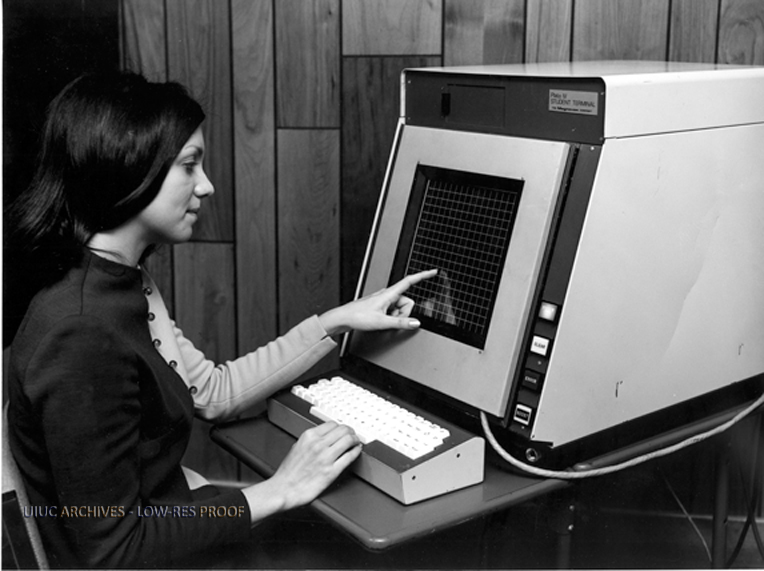
\includegraphics[width=0.8\textwidth] {bilder/platoiv.jpg}
\caption{Student using the PLATO IV.}
\label{platoIV}
\end{figure}
% Bild på xerox-musen eller mac-musen
%\nocite{platoiv}

%These devices used METOD - PROBLEM MED DETTA - BESKRIVA NÄSTA GENERATION. (DET SKA HANDLA OM LJUS HÄR, JAG REFERERAR TILL DETTA OSKRIVNA STYCKE SENARE.

The initial uses of touchscreens were point-to-select systems used in for example ATM machines or cash registers in restaurants and were relatively non-demanding on the screen performance\cite{buxton}. But there were also early attemps to make \emph{PDAs}\footnote{Personal Digital Assistant}. The first products to enter the market were the Palm Zoomer and the IBM Simon. The Simon was a mobile phone without any physical buttons, having only a touchscreen as its working area. But beyond regular telephone capabilities, it could also manage information such as a telephone book and be used for drawing and taking notes. Due to this, it is sometimes refered to as the first \emph{smartphone}\cite{buxton}.

Smartphones have seen much development since the release of Simon, and today (2013) it is estimated that more than a billion people use smartphones\cite{billion1}\cite{billion2}. [KORT STYCKE MED REFERENS SOM SÄGER ATT DET ÄR PGA ANDROID OCH IOS]. 

This increase in the number of touch-based devices has changed the way in which we interact with computers. New operating systems especially designed for smartphones and other smart devices, such as the popular IOs and Android operating systems have a fundamentally different approach to computer interaction.

The traditional WIMP approach requires the user to find the cursor on the display, move it to the desired location and click the mouse button to interact, or use the keyboard to input data. The touch screen on the other hand gives the user the ability to point directly at the desired item at the screen to activate it. An on-screen keyboard appears only when it is needed, allowed the computers to show only what is relevant at any point of time. This has made computers so portable that they can be used in almost any context and in a user friendly way [JAG TROR JAG KAN HITTA EN BRA REFERENS I MIN HCI-BOK]. The tablet is so simple in its design that it can be used by small kids and even cats [Bild på frasse tagen med en smartphone. Prata om att smart devices gör saker som att ta bilder].

%Multitouch. Vad är det, och varför?
One of the big breakthroughs that has allowed the touch screen to become the only input device required by a computer is the introduction of multi finger gestures. While touch screens previously only handled one action ("left mouse button"), the use of multi hand gestures removes the need for "icons" [DET FANNS ETT BRA ORD I NÅN ARTIKEL, HITTA!]. The rest of the functionality can be reached by for example pinching or swiping one's fingers. This type of interaction is not fundamentally more user-friendly, but it can be if used in the right way.

\begin{figure}[]
\includegraphics[width=0.8\textwidth] {bilder/ipadbook.jpg}
\caption{Apple Ipad showing iBooks, with the book Alice's Adventures in Wonderland.}
\label{ibooks}
\end{figure}
% Bild på xerox-musen eller mac-musen
\nocite{ipadbook}

Consider the common act of reading an e-book on a tablet. On a traditional computer, one typically reads the e-book as a document, with all pages following each other from top to bottom. On the tablet, the e-book can be made to look like a book, see figure \ref{ibooks}. The act of swiping one's finger from right to left triggers the book to turn the page, similar to what one would do in a physical book. This could be done with another gesture, for example by drawing a circle on the screen or triple-tapping an so on, but these approaches would not at all be as intuitive as the swipe-gesture.


\subsection{Voice recognition}

Voice recognition is another input method that has become increasingly popular during the last years. This input method uses speech recognition by analyzing input from a microphone. One the spoke word has been analysed, it can be used in several ways.

One ambition is that of providing real-time subtitles to spoken text, for example to aid those with hearing disorders. As an input method, the sound input can be parsed by the computer and then trigger a predefined action. In the past year (2012???????), Microsoft presented an English to synthesised speech Chinese translator, working in real time[CITATION NEEDED]. 



\subsection{Discussion}

% en diskussion och analys som sammanfattar båda ovanstående kategorier.